\documentclass[border=2mm]{standalone}

\usepackage{fontspec}
\usepackage{unicode-math}
\usepackage{amsmath}

\usepackage{pgfplots}
\pgfplotsset{compat=1.18}
\usetikzlibrary{arrows.meta, 
  calc, 
  positioning, 
  3d,
  decorations.pathreplacing, 
  calligraphy}
\usetikzlibrary{patterns}

\usepackage{xcolor}
\definecolor{den-1}{HTML}{111111}   % Đen #111111
\definecolor{den-2}{HTML}{222222}   % Đen #222222
\definecolor{den-3}{HTML}{333333}   % Đen #333333
\definecolor{den-4}{HTML}{444444}   % Đen #444444
\definecolor{den-5}{HTML}{555555}   % Đen #555555
\definecolor{den-6}{HTML}{666666}   % Đen #666666


\begin{document}

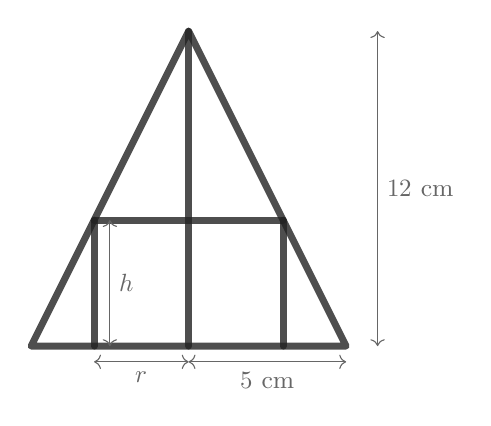
\begin{tikzpicture}[scale=1, line cap=round, line join=round]

  \draw[line width=2.5pt, color=den-2, opacity=.8] (-2,-4) -- (0,0) -- (2,-4) -- cycle;
  
  \draw[line width=2.5pt, color=den-2, opacity=.8] (-1.2,-2.4) -- (-1.2,-4);

  \draw[line width=2.5pt, color=den-2, opacity=.8] (1.2,-2.4) -- (1.2,-4);

  \draw[line width=2.5pt, color=den-2, opacity=.8] (-1.2,-2.4) -- (1.2,-2.4);

  \draw [line width=2.5pt, color=den-2, opacity=.8] (0,-4) -- (0,0);

  \draw [<->, color=den-6] (-1,-4) -- (-1,-2.4) node[midway, right] {\small $h$};

  \draw [<->, color=den-6] (2.4,-4) -- (2.4,0) node[midway, right] {\small $12 \text{ cm}$};

  \draw [<->, color=den-6] (-1.2,-4.2) -- (0,-4.2) node[midway, below] {\small $r$};

  \draw [<->, color=den-6] (0,-4.2) -- (2,-4.2) node[midway, below] {\small $5 \text{ cm}$};

\end{tikzpicture}


\end{document}
